\documentclass[a4paper]{article}
\usepackage{graphicx}
\graphicspath{/home/angelo/Documents/Uni/Courses/Advanced Statistics and programming/Assignments/assignment2/} 
\usepackage{mathtools}
\usepackage[a4paper, total={5in, 6.5in}]{geometry}
\usepackage{color}
\usepackage{tikz}
\usepackage{lipsum}
\usepackage{geometry}
\geometry{a4paper, left=2.5cm, top=2.5cm, bottom=2.5cm, right=2.5cm}
\usepackage{changepage}
\usepackage{booktabs}
\usepackage[font=small]{caption}
\DeclareCaptionFormat{mycaptionfont}{\fontsize{12}{13}\selectfont#1#2#3}
\usepackage{threeparttable}
\usepackage{ntheorem}
\usepackage{caption}
\usepackage{wrapfig,lipsum,booktabs}
\usepackage{listings}
\usepackage{pdflscape}
\captionsetup{format=mycaptionfont}
\usepackage{subcaption}
\theoremseparator{:}
\usepackage{lscape}
\usepackage{rotating}
\usepackage[utf8]{inputenc}
\newtheorem{hyp}{Hypothesis}
\usetikzlibrary{shapes,decorations,arrows,calc,arrows.meta,fit,positioning}
\tikzset{
    -Latex,auto,node distance =1 cm and 1 cm,semithick,
    state/.style ={ellipse, draw, minimum width = 0.7 cm},
    point/.style = {circle, draw, inner sep=0.04cm,fill,node contents={}},
    bidirected/.style={Latex-Latex,dashed},
    el/.style = {inner sep=2pt, align=left, sloped}
}





\begin{document}

\title{ASAP Assignment 3}
\author{Angelo Barisano; 508903 }
\date{October 10th, 2022}
\maketitle

\newpage
\section{Part 1}

\subsection{Task 1: Select Variables \& Names + Population regression equation}

\paragraph{No model without theory} The explanation of the quality of trade conditions in countries is closely tied to the overall development of countries. Slow cross border movements and transprtation times are an indicator for various problems that countries show in addition to a proxy for development adn furture development prospects. For instance, transporting one lorry from \textbf{CHAD} to the neighboring Niger takes about six times longer than the transport of the same lorry from Niger to France. 

In order to explain the quality of trade conditions, the time to export a good from a country is one possible outcome to be considered. Considering possible causal variables, exports as a percentage of GDP, industrial goods as a percentage of GDP, and GDP per capita are supported by theory. 
Firstly, more exports might lead to congestion at export hubs, such as harbors. Secondly, industrial goods are commonly associated with the development and export orientation of a country. Finally, GDP per capita is a commonly accepted measure of how good an economy is. For instance, Texas has the same GDP as Russia, but displays a considerably higher GDP per capita. GDP per capita is an accepted measure of economy efficiency and performance (Morgan \& Winship, 2015). 

Subsequently, that has lead to the proposed population equation to be created, explainaing time to export as a function of  exports as a percentage of GDP, industrial goods as a percentage of GDP, and GDP per capita:

$$ (1-1)   \\\   {Time To Export} = \alpha + \beta_{1}  Exports pct GDP + \beta_{2} Industry pct GDP + \beta_{3} GDP per Capita + \epsilon$$




\paragraph{THE NODE GRAPH AS IN ASSIGNMENT 1}
\begin{center}
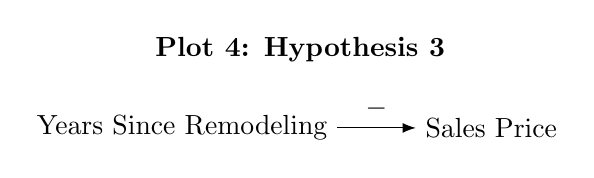
\begin{tikzpicture}
	\centering
 	\node at (1.5,1) {\textbf{Plot 4: Hypothesis 3}};
	\node (1) at (0,0) {Years Since Remodeling};
	\node (2) [right = of 1] {Sales Price};

	\path (1) edge node[above] {$-$}(2);
\end{tikzpicture}
\end{center}


\subsection{Task 2: Balance data \& descriptive statistics}

% Table created by stargazer v.5.2.3 by Marek Hlavac, Social Policy Institute. E-mail: marek.hlavac at gmail.com
% Date and time: Sun, Oct 09, 2022 - 17:49:53
\begin{table}[!htbp] 
\begin{adjustwidth}{-0cm}{-0cm}
\begin{threeparttable}
\small
\captionsetup{font=small, justification=raggedright,singlelinecheck=false}
  \caption{Panel Regression - Descriptive Statistics for Time to Export explanation} 
  \label{} 
\begin{tabular}{@{\extracolsep{5pt}}lccccccc} 
\\[-5.8ex]\hline 
\hline \\[-1.8ex] 
Statistic & \multicolumn{1}{c}{Mean} & \multicolumn{1}{c}{St. Dev.} & \multicolumn{1}{c}{Min} & \multicolumn{1}{c}{Pctl(25)} & \multicolumn{1}{c}{Median} & \multicolumn{1}{c}{Pctl(75)} & \multicolumn{1}{c}{Max} \\ 
\hline \\[-1.8ex] 
Year & 2,016.500 & 1.709 & 2,014 & 2,015 & 2,016.5 & 2,018 & 2,019 \\ 
Time to Export & 55.883 & 59.289 & 0.000 & 10.000 & 44.500 & 80.000 & 515.038 \\ 
GDP per Capita & 13,938.900 & 18,805.970 & 278.203 & 2,185.123 & 5,480.699 & 16,840.030 & 108,570.000 \\ 
Exports\_pct\_GDP & 42.212 & 31.551 & 0.611 & 23.167 & 34.711 & 49.795 & 213.090 \\ 
Industry\_pct\_GDP & 25.837 & 10.783 & 4.556 & 18.813 & 24.452 & 30.558 & 70.549 \\ 
\hline \\
[-3.5ex] 
\end{tabular} 
\begin{tablenotes}[para,flushleft]
      \small
      \item\textit{Notes:} N = 160 countries over 6 years resulting in 960 balanced observations
    \end{tablenotes}
\end{threeparttable}
\end{adjustwidth}
\end{table}

Table 1 contains the descriptive statistics for the balanced dataset regarding 160 full countries over six years each, ranging from 2014 to 2019. The total number of observations is consequently 960.
Considering the four variables contained in this analysis, time to export \textbf{in median days}, as an indicator of the quality of trade in a particular country, displays a mean of 55.88 \textbf{days} and a standard deviation of 59.289. While this might appear high in an European context, free trade is not universal and is also dependent on the infrastructure next to customs control. Overall, 50\% of all countries (median) display 44.5 \textbf{days} or less of time to export in addition to the 75th percentile staying at 80 \textbf{days}. This suggests, that few outliers cause a strong skewness of 2.673.

Following, GDP per capita displays a mean of \$13,938.90 ($std$ = 18,805.970) with a median of 5,480.70 again being lower than the mean, underlying the strong skewness of 2.144 of this variable. This is also to be expected considering the financial nature of the variable in addition to very few countries being quite rich when compared to other countries; ranging from \$278.17 to \$108,570.00.

Export as a percentage of GDP displays a mean on 42.212\% with a reasonably strong deviation of 31.551\% suggesting that certain countries, as with GDP per capita, display a stronger tendency to exporting and trading - thereby potentially disclosing a stronger tendency for efficient trade than others with lower percentages. Consequently, as the median is again lower than the mean ($median$ = \%34.711), this explains the strong positive skewness of the distribution of 2.508. The phenomenon of certain countries exporting more goods and services than their entire GDP ($max$ = 213.09\%) can originate for instance originate from this country being a transit state. Finally, industrial output as a percentage of GDP displays a mean of 25.84\% ($std$ = 10.783 ,$median$ = \%24.452).

It was decided for this exercise to not apply logscaling to those variables with strong skewness for three reasons: 1) logscaling might in certain circumstances increase the difficulty in interpretation, 2) in addition to potentially biasing the estimate of the coefficient ($exp(ln(Y) \neq Y$); particularly, both industry and exports as a percentage of GDP are already in the unit  percentages, which increases the difficulty in explaining these factors if logscaled. 3) Finally, these results are caused by normal outliers in the distribution which can be explained considering the reasonably small size in observations.

\subsection{Task 3: Perform the Regression}

Please note that the PLM package was ised for the calculation of the regressions in order to create comparability. Only the "within" model displayed minor differences in the estimation of the standard errors when compared to the manual "within" model, which was to be expected.



% Table created by stargazer v.5.2.3 by Marek Hlavac, Social Policy Institute. E-mail: marek.hlavac at gmail.com
% Date and time: Sun, Oct 09, 2022 - 19:01:06
% Requires LaTeX packages: dcolumn 
% Table created by stargazer v.5.2.3 by Marek Hlavac, Social Policy Institute. E-mail: marek.hlavac at gmail.com
% Date and time: Sun, Oct 09, 2022 - 19:02:17
\begin{table}[!htbp] 
\begin{adjustwidth}{-0cm}{-0cm}
\begin{threeparttable}
\small
\captionsetup{font=small, justification=raggedright,singlelinecheck=false}
  \caption{Regression Outputs for Pooled, Between, Within (FE), Random FE} 
  \label{} 
\begin{tabular}{@{\extracolsep{0pt}}lcccc} 
\\[-5.8ex]\hline 
\hline \\[-1.8ex] 
 & \multicolumn{4}{c}{\textit{Dependent variable:}} \\ 
\cline{2-5} 
\\[-1.8ex] & \multicolumn{4}{c}{TimeToExport} \\ 
\\[-1.8ex] & Pooled (1) & Between (2) & Within (3) & Random FE(4)\\ 
\hline \\[-1.8ex] 
 Constant & 44.375$^{***}$ & 43.034$^{***}$ &  & 68.107$^{***}$ \\ 
  & (5.058) & (12.438) &  & (6.871) \\ 
  Exports\_pct\_GDP & $-$0.177$^{***}$ & $-$0.173 & $-$0.030 & $-$0.146$^{*}$ \\ 
  & (0.063) & (0.154) & (0.108) & (0.087) \\ 
  Industry\_pct\_GDP & 1.277$^{***}$ & 1.325$^{***}$ & $-$0.234 & 0.195 \\ 
  & (0.161) & (0.395) & (0.216) & (0.185) \\ 
  GDPcap & $-$0.001$^{***}$ & $-$0.001$^{***}$ & 0.0001 & $-$0.001$^{***}$ \\ 
  & (0.0001) & (0.0003) & (0.0004) & (0.0002) \\ 
 \hline \\[-1.8ex] 
Observations & 954 & 159 & 954 & 954 \\ 
R$^{2}$ & 0.188 & 0.198 & 0.002 & 0.023 \\ 
Adjusted R$^{2}$ & 0.186 & 0.182 & $-$0.201 & 0.020 \\ 
F Statistic & 73.406$^{***}$ (df = 3; 950) & 12.730$^{***}$ (df = 3; 155) & 0.590 (df = 3; 792) & 22.621$^{***}$ \\ 
\hline 
\hline \\
[-3.5ex] 
\end{tabular} 
\begin{tablenotes}[para,flushleft]
      \small
      \item\textit{Notes:} N = 160 countries over 6 years resulting in 960 balanced observations. Non-robust standard errors are applied.
    \end{tablenotes}
\end{threeparttable}
\end{adjustwidth}
\end{table}

Table 2 contains the regression outputs for the pooled, between, within (of fixed effect), and random fixed effect model successively. All models, except for the fixed effect model (within) display a significant partial F test of the model ($F$ = 73.406, $p$ $<$ 0.01; $F$ = 12.730, $p$ $<$ 0.01; $F$ = 0.590, $p$ $=$ .622; $F$ = 22.621, $p$ $<$ 0.01), which is a test of the model specification itself.
The insignificant partial F test for the fixed effect model (this also applies to the "manually de-meaned" fixed effect model) suggests that the chosen variables do not correlate strongly with the time to export. However, this does not automatically suggest that the fixed effect model is not preferred over the pooled or between model as this requires a different kind of test - it may only be an indication. \textbf{Moreover, the partial F test of model significance only tests whether the proportion of between and within residuals are significantly different from each other: thus, the casual variables specified in task 1 may just not be correlated strongly on the country level with time to export; thus, this insignificant F test does not suggest that there are no country fixed effects at work here. }

Considering the model outputs, the pooled regression (or just OLS) model (1) displays that all three proposed causal variables are significant. As was expected, one percent more in exports as a percent of GDP leads to a reduction in time to export of \textbf{0.177} days ($p$ $<$ 0.01). GDP per capita also displays an expected negative relationship, where an increase of one USD in GDP per capita leads to a a reduction in time to export of 0.001 days ($p$ $<$ 0.01). Obviously, the effect sizes are not comparable due to the large difference in scales - GDP per capita vs industrial outputs as a percentage of exports are vastly different as can be seen in table 1.
However, contrary to the suggested association in task 2, an increase in industry output as a percentage of GDP by one percent leads to an increase in time to export \textbf{in days} by 1.28 ($p$ $<$ 0.01). Finally, GDP per capita displays a 

The between effects model compares the "over time aggregates" per country - the "between" entities part in the pooled model. In this context, the effect of export percentage in GDP is insignificant ($\hat{\beta}$ = -0.173, $p$ $=$ 0.263). Industrial output as a percentage of GDP ($\hat{\beta}$ = 1.325, $p$ $<$ 0.01) and GDP per capita ($\hat{\beta}$ = -0.001, $p$ $<$ 0.01), however, display a similar direction and effect as in the pool model. More importantly, the magnitude for the described effects, including exports as a percentage of GDP, is very similar to the coefficients in the pooled model. (foreshadowing) This indicates that the pooled model puts more "weight" on the between component of the model than the within component, which might explain the insignificant partial F test of the within (fixed effects) model. 

Thus, when moving on to the fixed effect model (3) in table 2, unsurprisingly, 1) there is no constant estimate, as we estimate a constant per country. Additionally, 2) as the insignificant partial F test indicated before, none of the defined causal variables display even a marginally significant relationship with time to export when observed on the country level only (Export \%: $\hat{\beta}$ = -0.030, $p$ $=$ 0.781; Industry \%: $\hat{\beta}$ = -0.216, $p$ $=$ 0.278; GDPpcap: $\hat{\beta}$ = 0.0001, $p$ $=$ 0.836). This might be explained by the similarity of the between and pooled model outputs mentioned above, not weighting the expected country specific time invariant factors, which might be to be expected; one such example might be corruption levels, where be can assume that those factors stay constant over time.
\textbf{However, when examining the intercepts for each country, one can see that most intercepts are significantly different from each other in time to export. This might indicate that there are underlying time fixed effects. However, the given causal variables seem to not predict any of the country specific factors.}


\textbf{MEntion the assumtions of within model here !!!}

Finally, considering the random fixed effect model, we can observe that GDP per capita is significant at conventional levels, displaying a negative (assumed) relationship with time to export ($\hat{\beta}$ = -0.001, $p$ $<$ 0.01); similar to the results of the pooled and between model. Additionally, the direction of the assumed effect is also similar for exports as a percentage of GDP - though only marginally significant at the ($p-value$) 9.4\% level ($\hat{\beta}$ = -0.146). Industrial output as a percentage of GDP was insignificant ($\hat{\beta}$ = 0.195, $p$ $=$ p = 0.293).
\textbf{DESCRIBE ASSUMPTIONS THAT GO INTO THE RANDOM FIXED EFFECT MODEL AND WHY TO USE THIS ONE POTENTIALLY!!}


It may be noted that the R²s' of the different models are not comparable as they resemble different estimation techniques; The fixed effect model also does not have a "typical" intercept, but rather multiple intercepts (one for each country). 


TO DO:
- explain why one would use the between, witin, random odel over others? 
- ALSO: hint at the intercepts. 



\subsection{WHICHM ODEL TO PREGFER}
to do:
- get all the intercepts to see whether within model is good or not
- do partial f test
- review the slides on this one!!!
- WHICH OF THE 4 models would you use in this context?!?!!?!!?!?!
- posisbly use plots!



%#' results: The constants are different for the random model (3) compared to pooled model (1)
%#' why? both use the same sources of varaition (within and between); but the pooled model uses OLS to estimate 
%#' and the random model uses generalized least squares, taking into account the panel data information (country and year) which is not
%#' taken into account in OLS! 
%#' SEE SLIDE 49 lecture 4 or 5 Random effects!!
%#' The reason why  you cannot use OLS is that the within group disturbances are probably autocorrelated!!!
%#' so you need to estimate this and take into account (ppoooled model does not do this )
%#' The generalized least squares (GLS) does this:
%#' What does the GLS do? it is the weighting of the within and between estimator!!!!(usngin both!!)
%#' 
%#' When to use random effects mode: 1) you use only fixed effects mdoel if you have reasons to beliefe 
%#' that there is some time constant unobserved factor such as culture (constant over time)in a country 
%#' influencing the explanatory variables 
%#' But if you do not have these concerns but special circumstances destroy the constant property within
%#' eg a country: we should use the random effects model because it also takes into account different sources of varaition
%#' the problem: random effects is notoften used

%# there is a test whether to use fixed vs random effects model
%# HAUSMAN TEST IS ALWAYS HELPFUL IN EVALUATING WHETHER TO USE one vs the other model!


%# Hausman test: compare random and fixed effects models.
%# Under H0, no correlation between disturbance and explana-
%# tory variables, both RE and FE are consistent (though FE
%# is not efficient), under H1, correlation between distur-
%# bance, only FE consistent
%phtest(rsltFE.Country, rsltRE.Country)

%#' hasuman test tests for significant differences between the coefficients of the two models
%#' if significant: prefer FIXED effect (test of one model (random effects) is inconsistent)
%#' if insignificant: USE RANDOM EFFECTS!!! (becasue the SE is too big! meaning that the coefficients and fixed effects
%#' vary too much in the fixed effects)






\section{Part 2 Count models}




\section{Part 3: Maximum Likelihood}





\end{document}
